\documentclass[10pt]{beamer}
\usetheme{CambridgeUS}
\usecolortheme{beaver}

\usepackage{pgfplots}
\usepackage{algorithm}
\usepackage{graphics}
\usepackage{graphicx}
\usepackage{amsmath}
\usepackage{mathtools}
\usepackage{algorithm,algorithmic}

\begin{document}

\title[Modeling OEC using EXAFS]{Modeling Metal Protein Complexes from Experimental Extended X-ray Absorption Fine Structure using Evolutionary Algorithms}

\author[Price \and Houghten \and Vassiliev \and Bruce]{
	Collin Price
	\and
	Sheridan Houghten
	\and
	Sergey Vassiliev
	\and
	Doug Bruce
}
\institute{Brock University}

% \begin{frame}

% \end{frame}

% \begin{itemize}
% 	\item 
% \end{itemize}

\begin{frame}
	\titlepage
\end{frame}

\section{Introduction}

\begin{frame}
	\frametitle{Outline}
	\tableofcontents
\end{frame}

\begin{frame}
	\frametitle{Cofactor}

	\begin{columns}[T]
		\begin{column}{.5\textwidth}
			\begin{itemize}
				\item ``helper'' molecules
				\item assist in biochemical transformations
				\item non-protein chemical compound
				\item exist within a protein
			\end{itemize}
		\end{column}
		\begin{column}{.5\textwidth}
			\begin{figure}
				\caption{Cofactor Examples}
				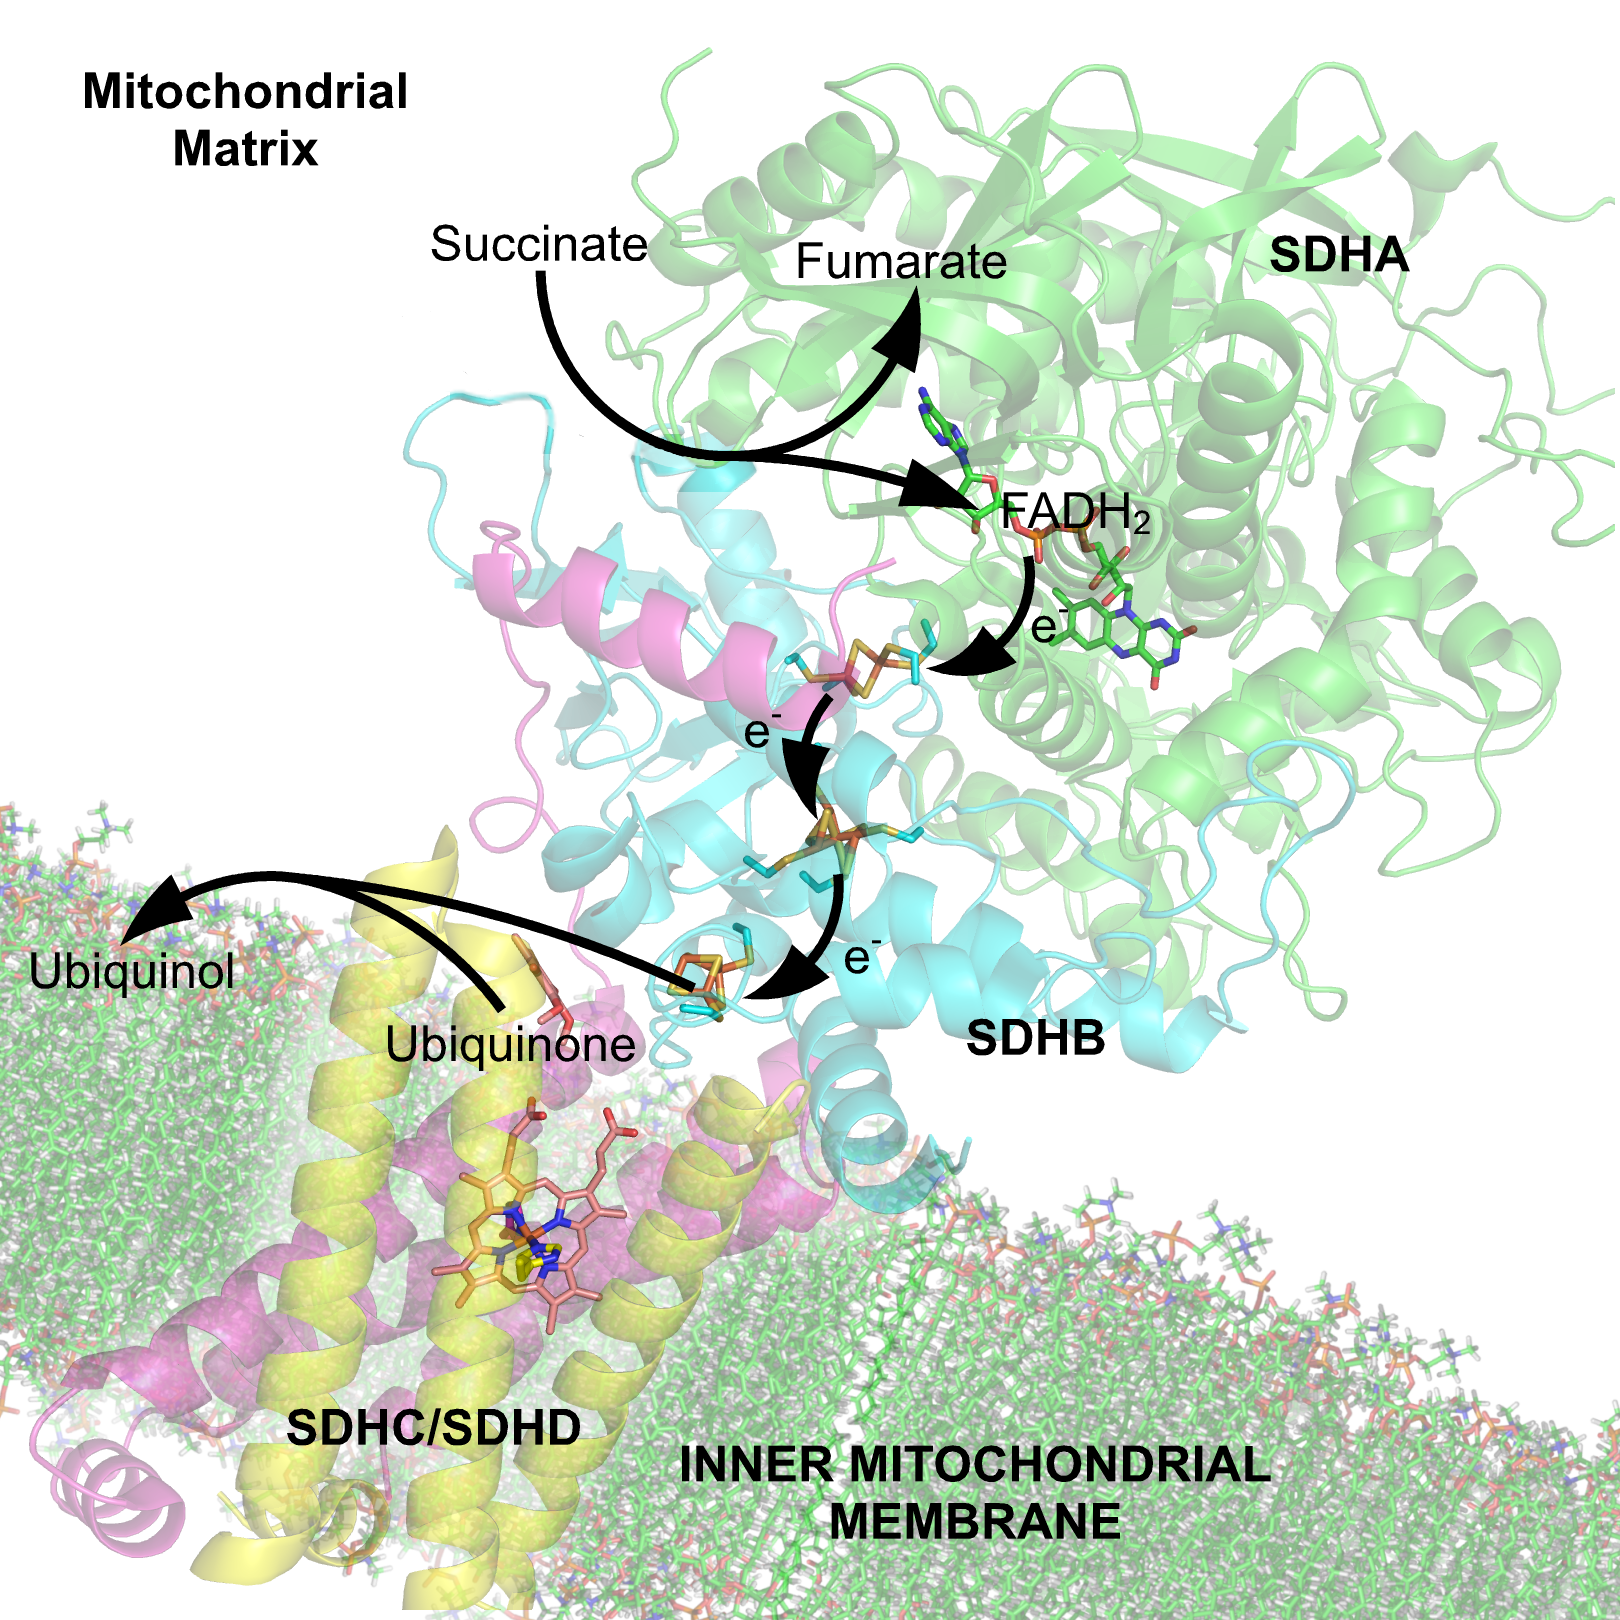
\includegraphics[width=1.0\textwidth,natwidth=1630,natheight=1620]{img/Succinate_Dehydrogenase_1YQ3_Electron_Carriers_Labeled.png}
			\end{figure}
		\end{column}
	\end{columns}
	
\end{frame}

\begin{frame}
	\frametitle{Oxygen-Evolving Complex (OEC)}

	\begin{columns}[T]
		\begin{column}{.5\textwidth}
			\begin{itemize}
				\item Water-splitting complex.
				\item Exists in 5 states: $S_{0}$ to $S_{4}$.
				\item Splits $H_{2}O$ into hydrogen and oxygen.
				\item $S_{4}$ reacts with water to produce oxygen.
				\item Process is not completely understood.
				\item $S_{1}$ is examined in this work.
			\end{itemize}
		\end{column}
		\begin{column}{.5\textwidth}
			\begin{figure}
				\caption{Metalloenzyme core of the OEC}
				
\includegraphics[width=1.0\textwidth,natwidth=620,natheight=485]{img/oec.png}
			\end{figure}
		\end{column}
	\end{columns}

\end{frame}

\begin{frame}
	\frametitle{Experimental Extended X-ray Absorption Fine Structure (EXAFS)}
	
	\begin{itemize}
		\item A method used to measure the absorption coefficient of a material as a function of energy.
		\item X-ray is tuned to have the same wavelength as the target atom.
			\begin{itemize}
				\item In the case of the OEC we targeted the four Manganese atoms.
			\end{itemize}
		\item X-ray reacts with target atom causing the atom to lose an electron and interact with neighbouring atoms.
		\item Fluorescence energies are emitted and measured.
	\end{itemize}

\end{frame}

\begin{frame}
	\frametitle{Experimental EXAFS Spectra}

	\begin{figure}
		\begin{tikzpicture}
		  \begin{axis}[
		    width=12cm,
		    height=6cm,
		    grid=both,
		    title={EXAFS Spectra in k space},
		    legend entries={Experimental},
		    legend pos=south east,
		    xlabel={$k \mathbin{/} A\textsuperscript{-1}$},
		    ylabel={$EXAFS \chi k\textsuperscript{3}$}
		  ]

		  \addplot[mark=x] table [col sep=comma,y index=1, x index=0] {results/best_run/for_chart.csv};

		  \end{axis}
		\end{tikzpicture}
		\caption{EXAFS Spectra of OEC in $S_{1}$}
	\end{figure}

\end{frame}

\begin{frame}
	\frametitle{Structure Refinement Problem}

	\begin{itemize}
		\item EXAFS spectra provides limited information about neighbouring atoms.
		\item We would like to know the 3-dimensional positions of each atom relative to each other.
		\item EXAFS spectra can be generated in simulations.
		\item If we match the calculated EXAFS spectra with the experimental EXAFS spectra it is likely we found the correct configuration.
		\item Goal is to minize the differences between spectra.
	\end{itemize}

\end{frame}

\begin{frame}
	\frametitle{Example Spectra Comparison}

	\begin{figure}
		\begin{tikzpicture}
		  \begin{axis}[
		    width=12cm,
		    height=6cm,
		    grid=both,
		    title={EXAFS Spectra in k space},
		    legend entries={Experimental,Calculated},
		    legend pos=south east,
		    xlabel={$k \mathbin{/} A\textsuperscript{-1}$},
		    ylabel={$EXAFS \chi k\textsuperscript{3}$}
		  ]

		  \addplot[mark=x] table [col sep=comma,y index=1, x index=0] {results/best_run/for_chart.csv};
		  \addplot[mark=*,mark size=1] table [col sep=comma,y index=2, x index=0] {results/best_run/for_chart.csv};

		  \end{axis}
		\end{tikzpicture}
		\caption{OEC EXAFS Spectra Comparison}
	\end{figure}

\end{frame}

\section{Previous Work}

\begin{frame}
	\frametitle{Previous Work}

	\begin{itemize}
		\item A model of the oxygen-evolving center of photosystem II predicted by structural refinement based on EXAFS simulations
			\begin{itemize}
				\item Sproviero, Eduardo M and Gasc{\'o}n, Jos{\'e} A and McEvoy, James P and Brudvig, Gary W and Batista, Victor S
				\item Quantum Mechanical and Molecular Mechanical hybrid
			\end{itemize}
		\item $S_{1}$-state model of the $O_{2}$-evolving complex of photosystem II
			\begin{itemize}
				\item Luber, Sandra and Rivalta, Ivan and Umena, Yasufumi and Kawakami, Keisuke and Shen, Jian-Ren and Kamiya, Nobuo and Brudvig, Gary W and Batista, Victor S
				\item Used a conjugate gradient optimization technique
				\item Monte Carlo
			\end{itemize}	
		\item Previous techniques would converge on local minima.
	\end{itemize}

\end{frame}

\section{Algorithms}

\begin{frame}
	\frametitle{Genetic Algorithm (GA)}

	\begin{itemize}
		\item Stochastic metaheuristic that mimics the process of natural evolution.
		\item A population of candidate solutions to an optimization problem are evolved toward better solutions.
		\item New candidates are created using crossover and mutation operators on existing candidate population.
	\end{itemize}
\end{frame}

\begin{frame}
	\frametitle{Restarting Genetic Algorithm (RGA)}

	\begin{itemize}
		\item Variation of the Recentering-Restarting Genetic Algorithm.
		\item Used to maintain diversity within the population.
		\item New candidate solutions are injected into the population once the convergence criteria is met.
	\end{itemize}
\end{frame}

\begin{frame}
	\frametitle{Restarting Genetic Algorithm}

	\begin{algorithm}[H]
		\caption{Restarting the population}
		\begin{algorithmic}[1]

		\IF{population has converged to minimum diversity}
		  \STATE remove all duplicate individuals;
		  \WHILE{population not full}
		    \STATE insert random draw from generated individuals into population;
		  \ENDWHILE
		\ENDIF

		\end{algorithmic}
	\end{algorithm}

\end{frame}

\begin{frame}
	\frametitle{Representation}

	\begin{columns}[T]
		\begin{column}{.6\textwidth}
			\begin{itemize}
				\item Set of 3-dimensional coordinates in space, where each position is assigned to a specific atom in the atomic structure.
				\item Entire OEC atomic structure contains 1269 atoms.
				\item EXAFS calculations only require 79 specific atoms.
				\item The units of measurement for each atom position are measured in Angstroms (\AA).
			\end{itemize}
		\end{column}
		\begin{column}{.4\textwidth}
			
			\begin{table}
				\caption{Example Chromosome}
				\begin{tabular}{ | c  c  c | }
					\hline
					$x_{0}$ & $y_{0}$ & $z_{0}$ \\ \hline
					$x_{1}$ & $y_{1}$ & $z_{1}$ \\ \hline
					$x_{2}$ & $y_{2}$ & $z_{2}$ \\ \hline
					$x_{3}$ & $y_{3}$ & $z_{3}$ \\ \hline
					... & ... & ... \\ \hline
				\end{tabular}
			\end{table}

		\end{column}
	\end{columns}

\end{frame}

\begin{frame}
	\frametitle{Population}

	\begin{itemize}
		\item Initial OEC atomic structure came from the crystallographic photosystem II structure in the Protein Data Bank.
		\item Randomly moving each atom produced too many unusable configurations.
		\item Needed to generate feasible structures for starting GA population.
		\item Used a molecular dynamics simulation to obtain these structures.
		\item Produces 10 000 atomic structures.
		\item Evaluated each and kept the top 300.
	\end{itemize}
\end{frame}

\begin{frame}
	\frametitle{Fitness}

	\begin{itemize}
		\item The goal of the experiment is to find an atomic structure that generates the same EXAFS spectra as the experimental EXAFS spectra.
		\item FEFF6 is used to simulate an XAFS experiment.
		\item IFEFFIT does post processing of the simulated EXAFS spectra.
		\item The root-mean-square deviations (RMSD) is used to calculate the difference between the experimental and calculated EXAFS spectra.
	\end{itemize}

	\begin{equation}
		RMSD = \sqrt{\frac{\sum_{t=1}^{n} \left ( x_{1,t}-x_{2,t} \right )^{2}}{n}}
	\end{equation}

\end{frame}

\begin{frame}
	\frametitle{Example Spectra Comparison}

	\begin{figure}
		\begin{tikzpicture}
		  \begin{axis}[
		    width=12cm,
		    height=6cm,
		    grid=both,
		    title={EXAFS Spectra in k space},
		    legend entries={Experimental,Calculated},
		    legend pos=south east,
		    xlabel={$k \mathbin{/} A\textsuperscript{-1}$},
		    ylabel={$EXAFS \chi k\textsuperscript{3}$}
		  ]

		  \addplot[mark=x] table [col sep=comma,y index=1, x index=0] {results/best_run/for_chart.csv};
		  \addplot[mark=*,mark size=1] table [col sep=comma,y index=2, x index=0] {results/best_run/for_chart.csv};

		  \end{axis}
		\end{tikzpicture}
		\caption{OEC EXAFS Spectra Comparison}
	\end{figure}

\end{frame}

\begin{frame}
	\frametitle{Operators}

	\begin{itemize}
		\item Crossover operator
			\begin{itemize}
				\item One-point crossover
			\end{itemize}
		\item Mutation operator
			\begin{itemize}
				\item Single atomic coordinate is randomly moved my 0.05\AA.
				\item Tested moving atomic coordinates by 0.001\AA, 0.005\AA, 0.01\AA, 0.025\AA, 0.05\AA, 0.1\AA, 0.5\AA, 1\AA, and 5\AA.
				\item 0.05\AA\ was chosen because it produced at least a 1\% change in fitness for all chemical elements.
			\end{itemize}
		\item Selection operator
			\begin{itemize}
				\item 3-tournament selection
			\end{itemize}
	\end{itemize}

\end{frame}

\section{Experiments}

\begin{frame}
	\frametitle{Experiment Setup}

	\begin{table}
		\caption{System Parameters used in GA and RGA}
		\begin{tabular}{ | l | r | }
		  \hline
		    Settings & Values \\ \hline \hline
		    Runs & 10 \\ \hline
		    Generations & Max. 30, Until Converged \\ \hline
		    Population Size & 50 \\ \hline
		    Crossover Rate & 80, 70 \\ \hline
		    Mutation rate & 10, 20, 30 \\ \hline
		    Elitism & True, False \\ \hline
		    Number of restart attempts & 3, 5 \\ \hline
		    Max convergence percentage before restarting & 5\%, 10\% \\ \hline
		\end{tabular}
	\end{table}
\end{frame}

\section{Results}

\begin{frame}
	\frametitle{Results from GA and RGA Experiments}

	% \begin{table}
	%   \caption{Results from GA and RGA Experiments}
	%   \begin{tabular}{ | l | l | l | l | l | l | l | l | l | l | }
	%     \hline
	%     Algo. & Gen. & Crossover & Mutation & Elitism & Conv. Rate & Restarting &  Avg. Best \\ \hline \hline
	%     GA & 30 & 80\% & 20\% & False & - & - & 1.3411 \\ \hline
	%     GA & 30 & 80\% & 10\% & False & - & - & 1.3746 \\ \hline
	%     GA & 30 & 70\% & 30\% & False & - & - & 1.2756 \\ \hline
	%     GA & 30 & 80\% & 10\% & True & - & - & 1.3278 \\ \hline
	%     GA & 30 & 70\% & 30\% & True & - & - & \textbf{1.2591} \\ \hline
	%     GA & 30 & 80\% & 20\% & True & - & - & 1.3299 \\ \hline
	%     RGA & 67 & 80\% & 20\% & True & 10\% & 3 & 1.2247 \\ \hline
	%     RGA & 81 & 80\% & 20\% & True & 5\% & 3 & 1.2117 \\ \hline
	%     RGA & 107 & 80\% & 20\% & True & 10\% & 5 & 1.2062 \\ \hline
	%     RGA & 124 & 80\% & 20\% & True & 5\% & 5 & 1.2156 \\ \hline
	%     RGA & 67 & 70\% & 30\% & True & 5\% & 5 & \textbf{1.1998} \\ \hline
	%     RGA & 81 & 70\% & 30\% & True & 10\% & 5 & 1.2138 \\ \hline
	%   \end{tabular}
	% \end{table}

	\begin{table}
	  % \caption{Results from GA Experiments}
	  \begin{tabular}{ | l | l | l | l | l | l | l | l | l | l | }
	    \hline
	    Gen. & Crossover & Mutation & Elitism & Conv. Rate & Restarting &  Avg. Best \\ \hline \hline
	    30 & 80\% & 20\% & False & - & - & 1.3411 \\ \hline
	    30 & 80\% & 10\% & False & - & - & 1.3746 \\ \hline
	    30 & 70\% & 30\% & False & - & - & 1.2756 \\ \hline
	    30 & 80\% & 10\% & True & - & - & 1.3278 \\ \hline
	    30 & 70\% & 30\% & True & - & - & \textbf{1.2591} \\ \hline
	    30 & 80\% & 20\% & True & - & - & 1.3299 \\ \hline
	  \end{tabular}
	\end{table}

	\begin{table}
	  % \caption{Results from RGA Experiments}
	  \begin{tabular}{ | l | l | l | l | l | l | l | l | l | l | }
	    \hline
	    Gen. & Crossover & Mutation & Elitism & Conv. Rate & Restarting &  Avg. Best \\ \hline \hline
	    67 & 80\% & 20\% & True & 10\% & 3 & 1.2247 \\ \hline
	    81 & 80\% & 20\% & True & 5\% & 3 & 1.2117 \\ \hline
	    107 & 80\% & 20\% & True & 10\% & 5 & 1.2062 \\ \hline
	    124 & 80\% & 20\% & True & 5\% & 5 & 1.2156 \\ \hline
	    67 & 70\% & 30\% & True & 5\% & 5 & \textbf{1.1998} \\ \hline
	    81 & 70\% & 30\% & True & 10\% & 5 & 1.2138 \\ \hline
	  \end{tabular}
	\end{table}

\end{frame}

\begin{frame}
	\frametitle{Results}

	\begin{figure}
		\begin{tikzpicture}
		  \begin{axis}[
		    grid=both,
		    title={Best RGA Run},
		    legend entries={Best,Average},
		    xlabel={Generations},
		    ylabel={RMSD}
		  ]

		  \addplot[mark=x] table [col sep=comma,y index=1, x index=0] {results/best_run/results-fixed.csv};
		  \addplot[mark=*] table [col sep=comma,y index=2, x index=0] {results/best_run/results-fixed.csv};

		  \end{axis}
		\end{tikzpicture}
		\caption{Example of a Restarting Genetic Algorithm}
	\end{figure}

\end{frame}

\begin{frame}
	\frametitle{Best RGA Spectra}

	\begin{figure}
		\begin{tikzpicture}
		  \begin{axis}[
		    width=12cm,
		    height=6cm,
		    grid=both,
		    title={EXAFS Spectra in k space},
		    legend entries={Experimental,Calculated},
		    legend pos=south east,
		    xlabel={$k \mathbin{/} A\textsuperscript{-1}$},
		    ylabel={$EXAFS \chi k\textsuperscript{3}$}
		  ]

		  \addplot[mark=x] table [col sep=comma,y index=1, x index=0] {results/best_run/for_chart.csv};
		  \addplot[mark=*,mark size=1] table [col sep=comma,y index=2, x index=0] {results/best_run/for_chart.csv};

		  \end{axis}
		\end{tikzpicture}
		\caption{OEC EXAFS Spectra Comparison}
	\end{figure}

\end{frame}

\begin{frame}
	\frametitle{Results}

	\begin{columns}[T]
		\begin{column}{.5\textwidth}
			\begin{itemize}
				\item GA and RGA were able to find a better solution than previously found.
				\item RGA was able to find a better solution than GA.
			\end{itemize}
		\end{column}
		\begin{column}{.5\textwidth}
			\begin{table}
				\caption{Comparison of Results}
				\begin{tabular}{ | l | l | l | l | l | }
				  \hline
				    Algorithm & Best Results \\ \hline
				    DFT-QM/MM & 1.2643 \\ \hline
				    R-QM/MM & 1.2403 \\ \hline
				    GA & 1.1452 \\ \hline
				    RGA & \textbf{1.0877} \\ \hline
				\end{tabular}
			\end{table}
		\end{column}
	\end{columns}

\end{frame}

\section{Post-Optimization}

\begin{frame}
	\frametitle{Post-Optimization}

	\begin{itemize}
		\item Results from GA and RGA were successful but we could do better.
		\item Convinced by guest speaker to try Particle Swarm Optimization.
		\item Convinced by fellow student to try Differential Evolution.
		\item Used the computational intelligence library, CILIB.
	\end{itemize}
\end{frame}

\begin{frame}
	\frametitle{Particle Swarm Optimization (PSO)}

	\begin{itemize}
		\item Better suited for continuous space problems.
		\item Contains a population of candidate solutions called particles.
		\item Particles move around the search space.
		\item Particles positions are updated based on the global best position and their local best position.
	\end{itemize}
\end{frame}

\begin{frame}
	\frametitle{Differential Evolution (DE)}

	\begin{itemize}
		\item Better suited for continuous space problems.
		\item Contains a population of candidate solutions called agents.
		\item An agents position is combined with other agents positions.
		\item If new agent is better, the old one is discarded.
	\end{itemize}
\end{frame}

\begin{frame}
	\frametitle{Population}

	\begin{itemize}
		\item Populations were initialized the same for both PSO and DE.
		% \item Molecular dynamics simulation used for GA/RGA could not be used for PSO and DE.
		\item Starting atomic structure was best found from RGA experiments.
		\item Generated population by randomly moving atomic coordinates by $\pm$0.05\AA\ and $\pm$0.25\AA.
	\end{itemize}
\end{frame}

\section{Experiments and Results}

\begin{frame}
	\frametitle{Results}

	\begin{table}
		\caption{Local Search Results}
		\centering
		\begin{tabular}{ | l | l | l | l | l | }
		  \hline
		    Algorithm & Initial Movement Radius & Pop. Size & Gen. & Average Best \\ \hline \hline
		    PSO & $\pm$0.05\AA & 50 & 30 & 0.8976 \\ \hline
		    DE & $\pm$0.05\AA & 50 & 30 & \textbf{1.1354} \\ \hline
		    PSO & $\pm$0.25\AA & 50 & 30 & 1.2411 \\ \hline
		    DE & $\pm$0.25\AA & 50 & 30 & 1.7220 \\ \hline \hline

		    PSO & $\pm$0.05\AA & 50 & 100 & \textbf{0.7782} \\ \hline
		\end{tabular}
	\end{table}

	\begin{itemize}
		\item DE was not able to improve upon previously found candidate solutions.
	\end{itemize}

\end{frame}

\begin{frame}
	\frametitle{Best Result}

	\begin{figure}
		\begin{tikzpicture}
		  \begin{axis}[
		    width=12cm,
		    height=6cm,
		    grid=both,
		    title={EXAFS Spectra in k space},
		    legend entries={Experimental, RGA Calculated, PSO Calculated},
		    legend pos=south east,
		    xlabel={$k \mathbin{/} A\textsuperscript{-1}$},
		    ylabel={$EXAFS \chi k\textsuperscript{3}$}
		  ]

		  \addplot[mark=x] table [col sep=comma,y index=2, x index=0] {results/pso_results/pso-100.csv};
		  \addplot[mark=-,mark size=1] table [col sep=comma,y index=2, x index=0] {results/best_run/for_chart.csv};
		  \addplot[mark=*,mark size=1] table [col sep=comma,y index=1, x index=0] {results/pso_results/pso-100.csv};

		  \end{axis}
		\end{tikzpicture}
		\caption{OEC EXAFS Spectra Comparison for PSO Post-Optimization}
	\end{figure}

\end{frame}

\begin{frame}
	\frametitle{Final Results}

	\begin{table}
		\caption{Comparison of Results}
		\begin{tabular}{ | l | l | l | l | l | }
		  \hline
		    Algorithm & Best Results \\ \hline
		    DFT-QM/MM & 1.2643 \\ \hline
		    R-QM/MM & 1.2403 \\ \hline
		    RGA & 1.0877 \\ \hline
		    PSO & \textbf{0.7287} \\ \hline
		\end{tabular}
	\end{table}

\end{frame}

\section{Subset Testing}

\begin{frame}
	\frametitle{Subset Testing}

	\begin{columns}[T]
		\begin{column}{.5\textwidth}
			\begin{itemize}
				\item Individuals contain 79 atoms.
				\item Wanted reduce the search space.
				\item Tested keeping certain chemical elements rigid during experiments.
			\end{itemize}
		\end{column}
		\begin{column}{.5\textwidth}
			\begin{table}
				\caption{Chemical Element Breakdown of OEC}
				\begin{tabular}{ | l | l | }
				  \hline
				    Element & Count \\ \hline
				    Mn & 4 \\ \hline
				    Ca & 1 \\ \hline
				    O & 26 \\ \hline
				    C & 14 \\ \hline
				    N & 6 \\ \hline
				    H & 28 \\ \hline
				    Total & 79 \\ \hline
				\end{tabular}
			\end{table}
		\end{column}
	\end{columns}

\end{frame}

\begin{frame}
	\frametitle{GA Parameters}

	\begin{table}
		\caption{GA Subset Parameters}
		\begin{tabular}{ l r }
		  \hline
		    Runs & 10 \\
		    Population size & 50 \\
		    Crossover rate & 0.7 \\
		    Mutation rate & 0.3 \\
		    Elitism & True \\
		    Number of restart attempts & 5 \\
		    Max convergence percentage before restarting & 5\% \\
		  \hline
		\end{tabular}
	\end{table}

\end{frame}

\begin{frame}
	\frametitle{Results}

	\begin{table}
		\caption{Results from subsets experiments}
		\begin{tabular}{ | l | l | l | }
			\hline
			Atoms & Best & Average \\ \hline \hline
			Mn, Ca, C, O, N, H & 1.1998 & 1.2580 \\ \hline
			Mn, Ca, C, O, N & \textbf{1.1697} & 1.2621 \\ \hline
			Mn, Ca, C & 2.4413 & N/A \\ \hline
			Mn, Ca, O & 1.2531 & N/A \\ \hline
			Mn, Ca, N & 2.4881 & N/A \\ \hline
			Mn, Ca, C, O & \textbf{1.1648} & N/A \\ \hline
			Mn, Ca, C, N & 2.5143 & 2.5649 \\ \hline
			Mn, Ca, O, N & N/A & N/A \\ \hline
			Mn, Ca & 2.4916 & 2.5088 \\ \hline
		\end{tabular}
	\end{table}

	Note: N/A means there were too many invalid solutions.

\end{frame}

\section{Conclusion and Future Work}

% \begin{frame}
% 	\frametitle{Conclusion}

% 	\begin{itemize}
% 		\item PSO significantly improved the solutions found by the RGA.
% 		\item DE performed poorly.
% 	\end{itemize}
% \end{frame}

\begin{frame}
	\frametitle{Future Work}

	\begin{itemize}
		\item Attempt direct comparison of PSO and DE with GA and RGA.
		\item Perform another molecular dynamics simulation on best result found from experimentation.
		\item Incorporate force fields into the algorithms to guarantee chemically feasible atomic structures.
		\item Multi-objective optimization using RMSD and potential energy.
	\end{itemize}
\end{frame}

\begin{frame}
	
	\begin{center}
	\Huge Questions?
	\end{center}

\end{frame}

\end{document}